\documentclass[12pt]{article}
\usepackage[onehalfspacing]{setspace}
\usepackage{dcolumn}
\usepackage[left=1in, top=1in, bottom=1in]{geometry}
\usepackage{graphicx}
\usepackage[table,xcdraw]{xcolor}
\usepackage{longtable}
\usepackage{float}
\usepackage{listings}
\usepackage{xcolor}
\usepackage{amsmath}
\usepackage{amsfonts}
\usepackage{amssymb}


\lstset{language=R,
    basicstyle=\small\ttfamily,
    stringstyle=\color{commentgreen},
    otherkeywords={0,1,2,3,4,5,6,7,8,9},
    morekeywords={TRUE,FALSE},
    deletekeywords={data,frame,length,as,character},
    keywordstyle=\color{blue},
    commentstyle=\color{commentgreen},
}
\begin{document}

\title{Syndicate 5 Statistical Learning Problem Set \#3}
\maketitle
{\setlength{\parindent}{0cm}


\section*{CD4 percentage level in child with HIV}
\subsection*{Question 1}
The model allowing for random effects on the intercept across different child patients can be modelled using the lme4 package to get the model below (see table 3 for more detail):

$$CD4PCT_i = \alpha_{j[i]} -3.3001 time_i + \epsilon_i$$
$$\alpha_j = 25.4729 + \eta_j \; \; \;\;\;\; \;\;\;\;\eta_j \sim N(0, \sigma^2_\alpha)$$

Looking at the fixed effects, the time predictor has a negative relationship with the percentage of CD4 cells. This makes sense, due to degenerative the nature of the disease, which kills CD4 cells over time. Holding everything else constant, for every year after the initial visit, the percentage of CD4 cells in an individual is estimated to reduce by 3\% per year. The intercept estimate ($\mu_\alpha$) was 25.47, indicating that at the start of the study (time=0) the average CD4 percentage reading across all patients was 25.47\%.\\


The random effects can be illustrated by plotting each patient coefficient ($\alpha_j$) with the average CD4 percentage reading ($\mu_\alpha$) as a baseline. The standard deviation at a 95\% confidence interval is also plotted for reference, refer to Figure 1. The plot (see Figure 1) shows significant variability between patients which is reflective of the high group variance of 130.25. This variability is likely attributed to the individual health and condition of the specific patient. Interestingly, patient specific variation is larger than idiosyncratic variation (11.413 vs 7.102).\\

The patient’s age at the start of the study, which may have some correlation with the severity of the disease, also differs across patients.  This would increase the variance in CD4 percentage readings across patients. Given this variability, it would be more appropriate to include treatment type and baseage of the patients to explain some of the variability. This will be explored further in question 2.


\subsection*{Question 2}
The model allowing for treatment and the child's age at their initial visit to explain the random intercept can be modelled using the lme4 package to give us the model below (see table 3 for more detail):

$$CD4PCT_i = \alpha_{j[i]} -3.2686 time_i + \epsilon_i$$
$$\alpha_j = 27.6231 + 1.9074 treatment_j -0.9259 baseage_j + \eta_j \; \; \; \; \; \; \eta_j \sim N(0, \sigma^2_\alpha)$$

In summary, while a child's CD4 percentage levels decrease over time, their initial levels are higher if the child had undertaken the new treatment course yet lower for groups (individual children) who started the treatment at older ages. Notably, while $time_i$ and $baseage_j$ are significant at the 1\% level, $treatment_j$ isn't even significant at the 10\% level so it likely has little effect on a child's base CD4 levels.\\


Plotting the child specific intercepts, we can see that the mean intercept for each child now changes depending on if they've undergone treatment and what their age was at the start of the treatment. Interestingly, patient specific variation is larger than idiosyncratic variation (11.220 vs 7.105).

\subsection*{Question 3}
The multiple linear model can be estimated using OLS as follows:
$$CD4PCT_i = 27.2739 -2.2862 time_i + 2.7089 treatment_j -0.9158 baseage_j + \epsilon_i$$
We determined that using patient ID as a categorical variable in the multiple linear model is not practical as it would create 226 dummy variables.\\

The multiple linear model treats each group (patient) the same and suggests that every patient has the same base CD4 levels as there is a fixed intercept for all groups. While this only ensures one source of randomness, from the individual level (cross-section), it gives us a different picture as to how factors such as treatment, time and base age affect a patient's CD4 levels. Notably, time seems to have less of an effect on CD4 levels in the multiple linear model than the multilevel model (-2.286 vs -3.269) while treatment has a greater effect (2.709 vs 1.907) while the effect of baseage is roughly the same (-0.916 vs -0.925).\\

In the multilevel regression model, the baseline of each group (patient) is allowed to be different. Thus, two sources of randomness are introduced. The first randomness occurs within groups, reflecting the effect of time. The second randomness comes between groups, allowing a different baseline, or initial condition, for each patient. Each patient’s personal situation and initial condition/baseline is different and the multilevel model accounts for this. Compared with the previous linear regression model, it is obvious that the multilevel regression model is more logical, practical, and informative.\\

This is further backed up by the AIC of this multiple linear regression model being 7813.825, which is significantly higher than the multilevel regression model with an AIC of 7146.052. Furthermore, the multilevel model is much more convenient than using 226 dummy variables with patient ID's.\\

In summary, the multilevel regression model is more valuable and informative compared with the multiple linear regression model.\\

\section*{Segments in the Credit data}
\subsection*{Question 1}
\subsubsection*{Present the Model}
Using the credit card data, the base linear model in Table 1 was generated assuming 2 components. For both components, the number of cards, marital status, gender and ethnicity did not have a statistically significant effect on credit card balance. Age was only significant for component 2, suggesting that age only had a negative relationship with balance for individuals in component 2. This difference was also highlighted in the sign direction of age for component 1, where the coefficient direction was positive rather than negative. Education was also only significant for component 2, however this significance level was quite weak at a level of 0.1. This suggests that level of education has a minor effect on balance for individuals in component 2 and no effect on individuals in component 1.\\

In both components, income, rating and student status was significant. The relationship of these predictors with balance was also consistent in direction. Hence, the overall relationship between the remaining statistically significant predictors and balance were as follows:\\
- Income had a negative effect on balance i.e. as income increased, the credit card balance decreased.\\
- Rating and whether the customer was a student had a positive effect on balance. 

\subsubsection*{Number of Clusters}
Three criteria are used for evaluation of different numbers of clusters: AIC, BIC and ICL (see table 4). As the result shown in Table 2, AIC is smallest (4528) when the model is associated with five clusters. Both BIC and ICL (4734 and 4851) are smallest when the model is associated with two clusters. For this model type, BIC is a better indicator than AIC as AIC tends to favour more complex models. The component size in this model is 84 for component 1 and 316 for component 2. Since component 1 is already quite small, it is also not favourable to reduce this group further. Hence, based on the BIC and the component size, the 2 component model is best suited for this analysis.
\begin{table}[H] \centering 
  \caption{Component 1} 
  \label{} 
\resizebox{11cm}{!}{

\begin{tabular}{@{\extracolsep{5pt}}lcccc} 
\\[-1.8ex]\hline 
\hline
\\ & Estimate & Std. Error & z-value & $Pr(>|z|)$\\ 
\hline \\[-1.8ex] 

(Intercept)       &  -369.57144  & 70.45484 & -5.2455 &1.559e-07 ***\\
Income            &    -7.48606  &  0.60733 &-12.3262 &$<$ 2.2e-16 ***\\
Rating            &     3.31753  &  0.13084 & 25.3550 &$<$ 2.2e-16 ***\\
Cards             &     8.66192  &  8.52800 &  1.0157 &   0.3098    \\
Age               &     0.19301  &  0.55350 &  0.3487 &   0.7273    \\
Education         &    -2.15821  &  3.67187 & -0.5878 &   0.5567    \\
StudentYes        &   526.35046  & 61.04724 &  8.6220 &$<$ 2.2e-16 ***\\
MarriedYes        &    -2.61280  & 19.99493 & -0.1307 &   0.8960    \\
GenderFemale      &    10.36153  & 18.42866 &  0.5623 &   0.5739    \\
EthnicityAsian    &    19.19905  & 27.63662 &  0.6947 &   0.4872    \\
EthnicityCaucasian&    12.00351  & 25.12970 &  0.4777 &   0.6329\\

\hline 
\hline \\[-1.8ex] 
\textit{Note:}  & \multicolumn{3}{r}{$^{*}$p$<$0.1; $^{**}$p$<$0.05; $^{***}$p$<$0.01} \\ 
\end{tabular} 
}
\end{table} 



\begin{table}[H] \centering 
  \caption{Component 2} 
  \label{} 
\resizebox{11cm}{!}{
\begin{tabular}{@{\extracolsep{5pt}}lcccc} 
\\[-1.8ex]\hline 
\hline
\\ & Estimate & Std. Error & z-value & $Pr(>|z|)$\\ 
\hline \\[-1.8ex] 


(Intercept)        &-785.457918 &  25.291452 &-31.0563 &$<$ 2.2e-16 ***\\
Income             &  -9.574878 &   0.195428 &-48.9944 &$<$ 2.2e-16 ***\\
Rating             &   4.738281 &   0.049802 & 95.1429 &$<$ 2.2e-16 ***\\
Cards              &   2.329100 &   2.333390 &  0.9982 &   0.3182    \\
Age                &  -1.121240 &   0.192084 & -5.8372 &5.307e-09 ***\\
Education          &   1.802016 &   1.094889 &  1.6458 &   0.0998 .  \\
StudentYes         & 468.483453 &  11.321723 & 41.3792 &$<$ 2.2e-16 ***\\
MarriedYes         & -11.580268 &   7.155990 & -1.6183 &   0.1056    \\
GenderFemale       &  -2.809011 &   6.899376 & -0.4071 &   0.6839    \\
EthnicityAsian     &   8.517622 &   9.642575 &  0.8833 &   0.3771    \\
EthnicityCaucasian &  -3.307501 &   8.159294 & -0.4054 &   0.6852    \\




\hline 
\hline \\[-1.8ex] 
\textit{Note:}  & \multicolumn{3}{r}{$^{*}$p$<$0.1; $^{**}$p$<$0.05; $^{***}$p$<$0.01} \\ 
\end{tabular} 
}
\end{table} 




\subsection*{Question 2}
\subsubsection*{Differences/similarities between Components}

Based on the chosen model, the summary statistics and coefficient comparisons in Table 5 and 6 were created. The median balance in component 1 was higher and had a larger range than component 2. The median income is slightly lower at \$32800 for component 1 than component 2 at \$36000. The effect of income is also higher in component 2 as indicated by the magnitude of the coefficient. Given these results, this could suggest that at higher income levels, the level of income has a higher negative effect on the credit card balance.\\

The median rating for both components is the same at 344 with a similar range, however, the effect of rating is higher for component 2. This suggests that whilst rating has a positive effect on balance in both groups i.e. balance increases with rating, this effect is greater for individuals in component 2.\\

The last remaining variable that was significant to both groups was whether the individual was a student. For both groups, if the individual was the student, this was associated with a higher balance. This effect was even higher for component 1, however this may be attributed to the lower proportion of students in this component.\\

Finally, the age predictor was only significant in component 2 and was estimated to have a negative relationship with balance i.e. as age increased, balance decreased. The median age was slightly lower for this group at 52 (compared to 56 in group 1), with a slightly smaller range of 24-91 compared to 23-98.\\


\subsubsection*{Key Differences between Week 1 and 5}
A key difference between this model and the models in week 1 and 5 (see table 7) is the variable selection. The week one model only has estimates for variables that were significant in our OLS estimate while also including squared terms for income and rating and the week 5 model copied these variables by design. The latent mixture model on the other hand contains variables that are statistically insignificant (at the 10\% level) in both components.\\

Week 1 only has one group of individuals suggesting that all of their balances behave in the same way, given a change in any of the variables included in the regression. Our latent mixture model suggests that an individual's balance can react in one of two ways, depending on what group they are in. The latent mixture model is likely to be more useful in this situation as balance behaviour is unlikely to be homogeneous.\\

Week 5 has the balance ratio as the dependant variable, not balance, which makes direct comparison difficult. The key difference here is that week 5's model censors balance ratios at the boundary (i.e. 0 and 1) whereas the latent mixture model doesn't do any censoring. For the case of modelling balance \textit{ratios}, the tobit model is more useful due to this feature, even if there isn't homogeneous balance behaviour.\\






\section*{Appendix}
Figure 1\\
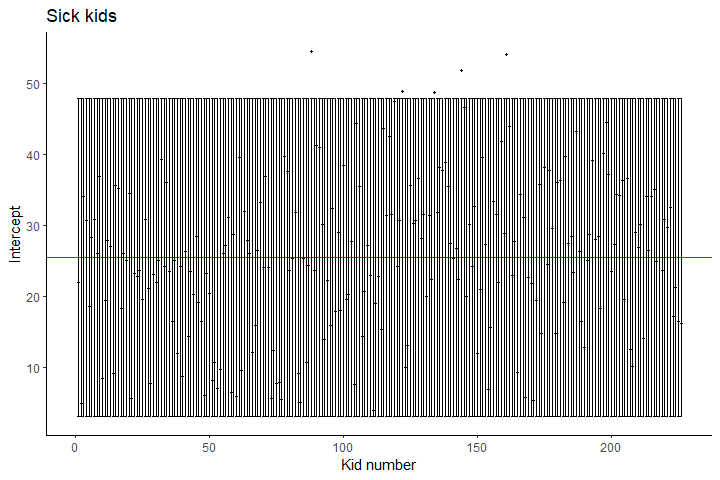
\includegraphics[scale=0.6]{Q1}\\
Figure 2\\
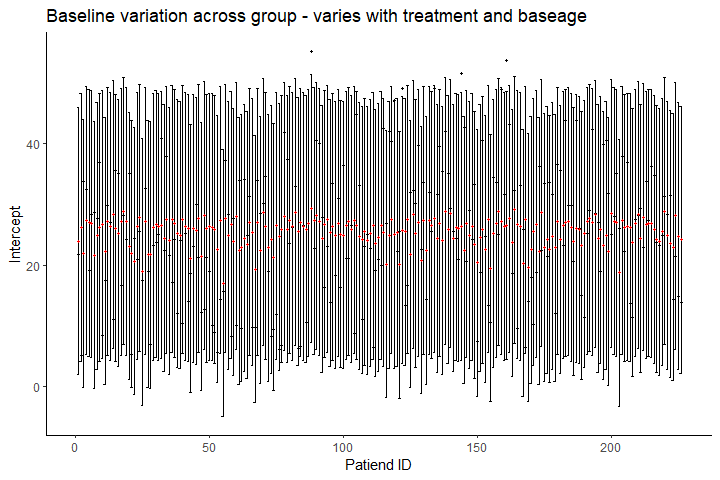
\includegraphics[scale=0.6]{Q2}\\



\begin{table}[!htbp] \centering 
  \caption{CD4PCT Regressions} 
  \label{} 
\begin{tabular}{@{\extracolsep{5pt}}lccc} 
\\[-1.8ex]\hline 
\hline \\[-1.8ex] 
 & \multicolumn{3}{c}{\textit{Dependent variable:}} \\ 
\cline{2-4} 
\\[-1.8ex] & \multicolumn{3}{c}{CD4PCT} \\ 
\\[-1.8ex] & \multicolumn{2}{c}{\textit{linear}} & \textit{OLS} \\ 
 & \multicolumn{2}{c}{\textit{mixed-effects}} & \textit{} \\ 
\\[-1.8ex] & (1) & (2) & (3)\\ 
\hline \\[-1.8ex] 
 time & $-$3.300$^{***}$ & $-$3.269$^{***}$ & $-$2.286$^{***}$ \\ 
  & (0.518) & (0.518) & (0.881) \\ 
  & & & \\ 
 treatment &  & 1.907 & 2.709$^{***}$ \\ 
  &  & (1.588) & (0.842) \\ 
  & & & \\ 
 baseage &  & $-$0.926$^{***}$ & $-$0.916$^{***}$ \\ 
  &  & (0.351) & (0.188) \\ 
  & & & \\ 
 Constant & 25.473$^{***}$ & 27.623$^{***}$ & 27.274$^{***}$ \\ 
  & (0.845) & (1.598) & (0.992) \\ 
  & & & \\ 
\hline \\[-1.8ex] 
Observations & 978 & 978 & 978 \\ 
R$^{2}$ &  &  & 0.041 \\ 
Adjusted R$^{2}$ &  &  & 0.038 \\ 
Log Likelihood & $-$3,572.420 & $-$3,567.026 &  \\ 
Akaike Inf. Crit. & 7,152.839 & 7,146.052 & 7813.825 \\ 
Bayesian Inf. Crit. & 7,172.381 & 7,175.365 &  \\ 
Residual Std. Error &  &  & 13.102 (df = 974) \\ 
F Statistic &  &  & 14.004$^{***}$ (df = 3; 974) \\ 
\hline 
\hline \\[-1.8ex] 
\textit{Note:}  & \multicolumn{3}{r}{$^{*}$p$<$0.1; $^{**}$p$<$0.05; $^{***}$p$<$0.01} \\ 
\end{tabular} 
\end{table} 

\begin{table}[H] \centering 
  \caption{} 
  \label{} 
\begin{tabular}{@{\extracolsep{5pt}}lccccccc} 
\hline \hline
iter & converged &k& k0   & logLik   &   AIC    &  BIC  &    ICL\\
\hline \\ 
    2   &   TRUE& 1 & 1& -2415.525& 4855.049& 4902.947& 4902.947\\
   25   &   TRUE& 2 & 2& -2292.172& 4634.345& 4734.131& 4850.949\\
   82   &   TRUE& 3 & 3& -2265.414& 4606.828& 4758.504& 4874.776\\
  200   &  FALSE& 4 & 4& -2242.471& 4586.942& 4790.507& 4948.840\\
  180   &   TRUE& 5 & 5& -2201.789& 4531.578& 4787.032& 5006.904\\
\hline 
\hline \\[-1.8ex] 
\end{tabular} 
\end{table} 

\begin{table}[H] \centering 
  \caption{Coefficient Comparison} 
  \label{} 
\begin{tabular}{l|ll}
\hline
\textit{\textbf{Coefficient}} & \textbf{Component 1} & \textbf{Component 2} \\
\hline
\textbf{Intercept} & (-) Lower Magnitude & (-) Higher Magnitude \\
\textbf{Income} & (-) Lower Magnitude & (-) Higher Magnitude \\
\textbf{Rating} & (+) Lower & (+) Higher \\
\textbf{Cards} & (+) Not Significant & (+) Not Significant \\
\textbf{Age} & (+) Not Significant & (-) Significant \\
\textbf{Education} & (-) Not Significant & (+) Not Significant \\
\textbf{Student==Yes} & (+) Higher & (+) Lower \\
\textbf{Married==Yes} & (+) Not Significant & (-) Not Significant \\
\textbf{Gender==Female} & (+) Not Significant & (-) Not Significant \\
\textbf{Ethnicity==Asian} & (+) Not Significant & (+) Not Significant \\
\textbf{Ethnicity==Caucasian} & (+) Not Significant & (-) Not Significant
\end{tabular}
\end{table}

\begin{table}[H] \centering 
  \caption{Summary Statistics (Numeric: Median, Min, Max, Categorical: Proportions)} 
  \label{} 
\begin{tabular}{l|ll}
\hline
\textit{\textbf{Coefficient}} & \textbf{Component 1} & \textbf{Component 2} \\
\hline
\textbf{Balance} & 465 (0, 2000) & 450 (0, 1780) \\
\textbf{Income} & 32.8 (10.4, 187) & 36.6 (10.6, 180) \\
\textbf{Rating} & 344 (93, 982) & 344 (126, 828) \\
\textbf{Cards} & 3 (1, 9) & 2 (1, 6) \\
\textbf{Age} & 56 (23, 98) & 52 (24, 91) \\
\textbf{Education} & 14 (5, 20) & 13 (6, 19) \\
\textbf{Student==Yes} & 0.093 & 0.148 \\
\textbf{Married==Yes} & 0.610 & 0.630 \\
\textbf{Gender==Female} & 0.514 & 0.537 \\
\textbf{Ethnicity==Asian} & 0.243 & 0.333 \\
\textbf{Ethnicity==Caucasian} & 0.500 & 0.481
\end{tabular}
\end{table}

\begin{table}[H] \centering 
  \caption{Week 1 and Week 5 Models} 
  \label{} 
\begin{tabular}{@{\extracolsep{5pt}}lcc} 
\\[-1.8ex]\hline 
\hline \\[-1.8ex] 
 & \multicolumn{2}{c}{\textit{Dependent variable:}} \\ 
\cline{2-3} 
\\[-1.8ex] & Balance & BalanceRatio \\ 
\\[-1.8ex] & (Week 1 Multiple) & (Week 5 Tobit)\\ 
\hline \\[-1.8ex] 
 Income & $-$6.238$^{***}$ & $-$0.002587$^{***}$ \\ 
  & (0.486) & (0.00009133) \\ 
  & & \\ 
 I(Income$\hat{\mkern6mu}$2) & $-$0.021$^{***}$ & 0.000005766$^{***}$ \\ 
  & (0.003) & (0.0000006255) \\ 
  & & \\ 
 Rating & 2.471$^{***}$ & 0.001159$^{***}$ \\ 
  & (0.136) & (0.00003103) \\ 
  & & \\ 
 I(Rating$\hat{\mkern6mu}$2) & 0.002$^{***}$ & $-$0.0000006128$^{***}$ \\ 
  & (0.0002) & (0.00000003681) \\ 
  & & \\ 
 Age & $-$0.729$^{***}$ & $-$0.0001993$^{***}$ \\ 
  & (0.261) & (0.00004925) \\ 
  & & \\ 
 StudentYes & 428.341$^{***}$ & 0.1018$^{***}$ \\ 
  & (14.755) & (0.002608) \\ 
  & & \\ 
 Constant & $-$329.576$^{***}$ & $-$0.1386$^{***}$ \\ 
  & (26.542) & (0.006190) \\ 
  & & \\ 
\hline \\[-1.8ex] 
Observations & 400 &  \\ 
R$^{2}$ & 0.964 &  \\ 
Adjusted R$^{2}$ & 0.963 &  \\ 
Residual Std. Error (df = 393) & 88.218 &  \\ 
F Statistic (df = 6; 393) & 1,740.723$^{***}$ & \\ 
\hline 
\hline \\[-1.8ex] 
\textit{Note:}  & \multicolumn{2}{r}{$^{*}$p$<$0.1; $^{**}$p$<$0.05; $^{***}$p$<$0.01} \\ 
\end{tabular} 
\end{table}


}
\end{document}